\chapter{Test Bed and Design Decisions}
\label{chap:testbed}

%%%%%%%%%%%%%%%%%%%%%%%%%%%%%%%%%%%%%
%%%%%%%%%%%%%%%%%%%%%%%%%%%%%%%%%%%%%
%%%%%%%%%%%%   SECTION   %%%%%%%%%%%%
%%%%%%%%%%%%%%%%%%%%%%%%%%%%%%%%%%%%%
%%%%%%%%%%%%%%%%%%%%%%%%%%%%%%%%%%%%%
\section{Pros and Cons of the Baseline Analysis}
\label{sec:mm:pros_n_cons}
The contribution of this thesis starts with scrutinizing the Baseline Analysis. Upsides and downsides are investigated and their validity are verified.
\subsection{Pros}
\label{mm:pros}
Baseline analysis has considered every possible delicate detail to compute the worst case execution time. Upsides of the analysis are discussed here.

\subsubsection{CPU Utilization Balancing}
In time partition scheme, CPU utilization factors for A/A mode and A/G mode can be well balanced by configuring time slot period. For instance, in space partition scheme, Core\#4 is utilized 75\% in A/A mode processing and 25\% in A/G mode processing. This information gives a hint for time partitioning that A/A mode needs more time span than A/G mode in Core\#4. It is adopted in Scheme-2, allocating 14.5ms for A/A mode and 4.5ms for A/G Mode to balance the CPU utilization. Dynamic partition configuration can be considered in future to improve CPU utilization balancing.

\subsubsection{Memory Partitioning}
In time partition scheme, shared resources (L2 cache, Memory) are partitioned for A/A Mode and A/G mode to provide segregation. This isolation clearly defines the accessible address space for each core. Even if A/G mode processing of a core consumes huge memory space, A/A mode data of the core remains intact and will be useful during the next time slice. Another advantage of memory partitioning is, it allows utilization balancing among the memory resources.

\subsection{Cons}
\label{mm:cons}
\subsubsection{Context Switch Time}
Context switch time of 0.5ms is assumed for time partitioning. Every core does 2 context switches in 20ms. In time partition analysis (Scheme-2), at the end of 19.50ms all the four cores want to perform context switching. It is illustrated in Figure \ref{fig:mm:mm_cons1}. Since the SDRAM has only one port, it is possible for only one core to access the memory. Other cores have to wait till that time. 

\begin{figure}[h!]
	\centering
	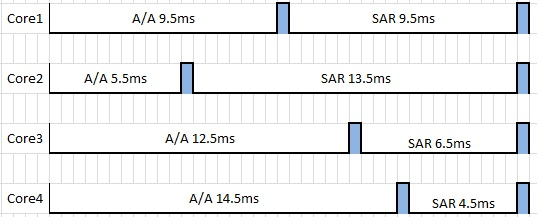
\includegraphics[width=120mm]{figures/mm_cons1}
	\caption{Time Partition of Scheme 3}
	\label{fig:mm:mm_cons1}
\end{figure}

Assuming the order of SDRAM access is Core\#1, Core\#2, Core\#3 and Core\#4. Core\#2 waits for Core\#1 to complete (0.5ms), Core\#3 waits for Core\#1,2 (0.5ms + 0.5ms), Core\#4 waits for Core\#1,2,3 (0.5ms + 0.5ms + 0.5ms). This overhead in waiting time sums up to 3ms. Though only one context switch is contending, during the course of run it will be a scenario where two context switches will contend for SDRAM because of its skewed timing behaviour. Worst-case waiting time for four cores is 
\begin{align*}
	& = \frac{4*T_{cs} \enspace + \enspace 2*T_{ow}}{T_{a}} \\[0.4cm]
	& = \frac{4*2*0.5ms \enspace + \enspace 2*3ms}{4*20ms} = 12.5\% \stepcounter{equation}\tag{\theequation} 
\end{align*}
\noindent
\textbf{Legend} \\
\tab $T_{cs}:$ Context-switch time \\
\tab $T_{ow}:$ Overhead in waiting time \\
\tab $T_{a}:$ Available time \\

In the worst case scenario, 12.5\% of the CPU time is spent only for context switching. This percentage is severe for a Radar processor. It degrades the application performance and much meaningful processing can be done during that time. \\

\textbf{\textsl{Verification:}} LMbench microbenchmark\cite{lmbench} is used to measure the context switch time of the ARM cores. LMbench is a free software suite of simple, portable benchmarks to compute various system performances including memory copy bandwidth, context switch latency, system call overhead, process creation latency, etc. Different sets of processes and data size are examined for the context switch time measurement. The LMbench suggests that the lowest recorded context switch time measurement is the more realistic one. So, lowest value of the 20 measurements are computed and listed in Table \ref{mm:ctxsw:lmbench}. 7.43$\mu$s in the table belongs to the context switch time measurement of two processes having 8KiB working data set each. The processes are scheduled according to the scheduling policy of the operating system. By monitoring the \verb|top| command, it is evident that the cores execute processes simultaneously, i.e. when four processes are involved in context switch, four cores are performing the execution.

\begin{table}[h!]
	\begin{tabularx}{\textwidth}{|X|X|X|X|X|}
		\hline
		\multirow{2}{*}{\textbf{Data Size [KiB]}} & \multicolumn{4}{c|}{\textbf{Context Switch Time[\boldmath$\mu$s]}} \\ \cline{2-5}
		& \textbf{2p} & \textbf{4p} & \textbf{8p} & \textbf{16p}  \\ \hline 
		8 & 7.43 & 9.09 & 12.76 & 13.58 \\ \hline
		16 & 8.22 & 16.35 & 19.31 & 20.87 \\ \hline
		32 & 9.57 & 18.48 & 23.68 & 29.13 \\ \hline
	\end{tabularx}
\caption{Measured Context Switch Time}
\label{mm:ctxsw:lmbench}
\end{table}

\begin{figure}[h!]
\centering
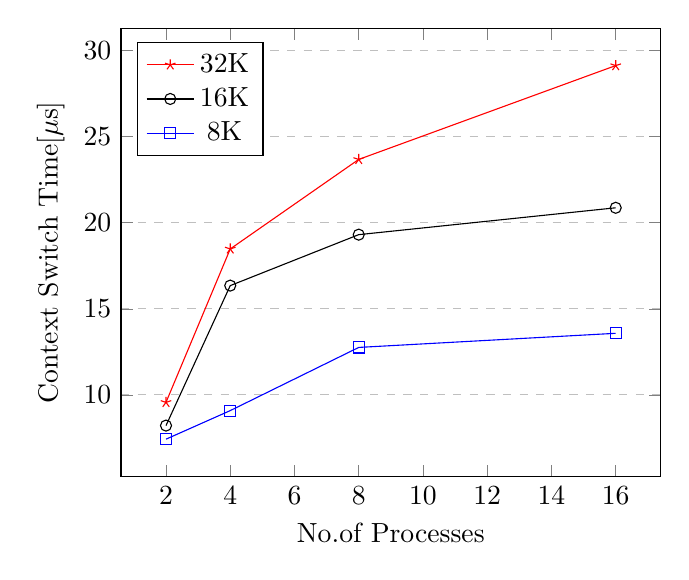
\begin{tikzpicture}
\begin{axis}[
	xlabel={No.of Processes},
	ylabel={Context Switch Time[$\mu$s]},
	legend pos=north west,
	ymajorgrids=true,
	grid style=dashed,
]
\addplot[color=red, mark=star,]
	coordinates {
		(2, 9.57) (4, 18.48) (8, 23.68) (16, 29.13)
	};

\addplot[color=black, mark=o,]
	coordinates {
		(2, 8.22) (4, 16.35) (8, 19.31) (16, 20.87)
	};
	
\addplot[color=blue, mark=square,]
	coordinates {
		(2, 7.43) (4, 9.09) (8, 12.76) (16, 13.58)
	};

	\legend{32K, 16K, 8K}
\end{axis}
\end{tikzpicture}
\caption{Comparison of Context Switch Time}
\label{mm:cntxt_switch_graph}
\end{figure}

From the above three sets of measurements, worst-case context switch time is 29.13$\mu$s corresponds to the 16 processes operating on 32KiB memory size. Also it reveals that the context switch time is proportional to the number of processes and data set size. On contrary to the assumption of 0.5ms context switch time and 12.5\% degradation in CPU utilization, measured worst-case context switch time is much lesser, therefore will not deteriorate the CPU utilization. So, no changes are made in the Baseline Analysis with respect to the context switch time.

\subsubsection{Clashing Data Streams}
In time partition scheme, assume that the Core\#1 of CPU1 is executing A/A Mode time slice. Now, A/G Mode data is routed to the same CPU by PSM2 as shown in Figure \ref{fig:mm:data_clash}. The core cannot accept the A/G Mode data as it is executing A/A time slice and the PSM have no idea of what the cores are up to or what to do with the data if the core is not accepting. This corner case is not clearly defined in the Baseline Analysis, as a result it leads to data loss if no countermeasure is provided.

\begin{figure}[h!]
	\centering
	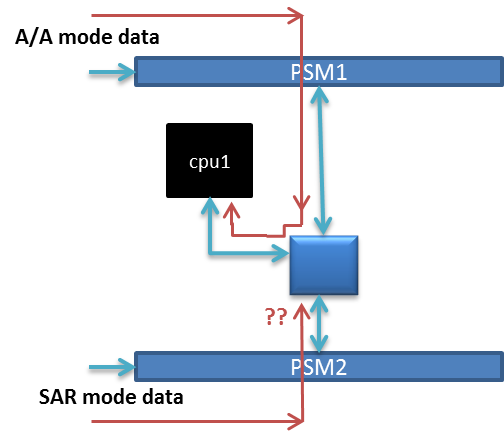
\includegraphics[width=80mm]{figures/data_clash}
	\caption{Clashing Data Streams}
	\label{fig:mm:data_clash}
\end{figure}

One of the ways to resolve this is to have a buffer in PSM to store the incoming data stream. If the core is not accepting the data, corresponding \verb|core_id| and \verb|cpu_id| shall be stored in the PSM along with the data. When the core is requesting data during next A/G Mode time slice, the PSM can transfer the stored data if the \verb|core_id| and \verb|cpu_id| matches. Since the incoming data stream is stored for one time slice period, it has to be counted for the processing latency calculation. The storing and restoring scheme ensures that the A/A data and A/G data will never be routed to the same CPU at the same time.

\subsubsection{Scalability}
\label{sss:mm:cons:scalability}
For time slot adjustment, it is cumbersome task to break the entire application into pieces such that each and every piece will fit in to one time slot. Whenever there is a change in time slot period, the entire application requires rework to suspend itself before the time slot expires. It implies that the time and cost of the application development and maintenance will increase. In addition, amendments are needed if the Radar configuration such as PRF set is changed.

\subsection{Other Comments}
\subsection{Measured Values of the Baseline Analysis}
\label{mm:cons:real_values}
The execution cycles of the functional blocks gives in the previous chapter (Table \ref{sec:ch2:benchmark_results}) were not the same when measured in a real hardware. The measured execution cycles are adapted in the Baseline Analysis and the results are presented here.

\subsubsection{Scheme-1}
\begin{table}[h!]
	\centering
	\begin{tabular}{|l|l|l|l|l|} 
	 \hline
	& \textbf{Core\#1} & \textbf{Core\#2} & \textbf{Core\#3} & \textbf{Core\#4} \\ \hline
	\textbf{Utilization} & 19.03\% & 46.20\% & 65.78\% & {\color{red} 108.07\%} \\ \hline
	\end{tabular}
	\caption{Measured CPU Utilization of Scheme-1, A/A Mode}
	\label{tbl:mm:scheme1_true_util}
\end{table}

\begin{table}[h!]
	\centering
	\begin{tabular}{|c|l|l|l|} 
	 \hline
	 \textbf{Look direction} & \textbf{Dwell time[ms]} & \textbf{Latency[ms]} & \textbf{\#Dwells transmitted} \\
	 \hline
	 1 & 27.84 & 416.40 & 14.96 \\ \hline
	 2 & 33.07 & 482.28 & 14.58 \\ \hline
	 3 & 39.17 & 574.52 & 14.67 \\ \hline
	 4 & 46.20 & 662.80 & 14.35 \\ \hline
	 5 & 54.26 & 798.62 & 14.72 \\ \hline
	\end{tabular}
	\caption{Measured Processing Latency of Scheme-1, A/A Mode}
	\label{tbl:mm:scheme1_true_latency}
\end{table}
Core\#4 of the A/A Mode processing CPUs in Scheme-1 required more than the available time to process one Burst of the input data. It leads to unfaithful result as it cannot cope up the incoming data stream.
\FloatBarrier

\subsubsection{Scheme-2}
\begin{table}[h!]
	\centering
	\begin{tabular}{|l|l|l|l|l|} 
	 \hline
	& \textbf{Core\#1} & \textbf{Core\#2} & \textbf{Core\#3} & \textbf{Core\#4} \\ \hline
	\textbf{Utilization} & 25.00\% & {\color{red} 103.33\%} & 71.43\% & 83.33\% \\ \hline
	\end{tabular}
	\caption{Measured CPU Utilization of Scheme-2, A/A Mode}
	\label{tbl:mm:scheme2_true_util}
\end{table}

\begin{table}[h!]
	\centering
	\begin{tabular}{|c|l|l|l|} 
	 \hline
	 \textbf{Look direction} & \textbf{Dwell time[ms]} & \textbf{Latency[ms]} & \textbf{\#Dwells transmitted} \\
	 \hline
	 1 & 27.84 & 860.00 & 30.89 \\ \hline
	 2 & 33.07 & 920.00 & 27.82 \\ \hline
	 3 & 39.17 & 1060.00 & 27.06 \\ \hline
	 4 & 46.20 & 1220.00 & 26.41 \\ \hline
	 5 & 54.26 & 1520.00 & 28.01 \\ \hline
	\end{tabular}
	\caption{Measured Processing Latency of Scheme-2, A/A Mode}
	\label{tbl:mm:scheme2_true_latency}
\end{table}
\FloatBarrier
Here, Core\#2 is utilized beyond its limits and the Dwell time latency reaches up to 30x Dwell time. Both the Schemes will not adhere to the real-time requirements.

%\clearpage
%%%%%%%%%%%%%%%%%%%%%%%%%%%%%%%%%%%%%
%%%%%%%%%%%%%%%%%%%%%%%%%%%%%%%%%%%%%
%%%%%%%%%%%%   SECTION   %%%%%%%%%%%%
%%%%%%%%%%%%%%%%%%%%%%%%%%%%%%%%%%%%%
%%%%%%%%%%%%%%%%%%%%%%%%%%%%%%%%%%%%%
\section{Test Procedure} 
\label{sec:mm:test_procedure}
A Nitrogen6X development kit is used to match the basic building block of the IMA processor architecture, which is iMX6Quad processor, clocked 1GHz. The communication to the Nitrogen6X board is carried via Ethernet interface. Measurements of the processing latency is performed on the target and exported in \bverb|.csv| format. The results are scaled down to 800MHz to match the IMA architecture. Scheduling schemes and processing latency analysis are based on the single iMX6Quad processor result, measured from the Nitrogen6X board.

%%%%%%%%%%%%%%%%%%%%%%%%%
%%%%%   SUB-SECTION   %%%
%%%%%%%%%%%%%%%%%%%%%%%%%
\subsection{Target Hardware}
\label{ss:bg_related_work:hw}
The target hardware is a Nirtogen6X development board (Appendix \ref{app:nitrogen6x}) from Boundary Devices Inc. It is a low cost development kit built with iMX6Quad processor. Some of it's features are:
\begin{compactitem} 
	\item Quad-Core ARM Cortex A9 processor clocked 1GHz
	\item 1GiB of 64-bit wide DDR3 at 532MHz
	\item Three display ports (RGB, LVDS and HDMI)
	\item Serial ATA 2.5 (SATA) at 3GBit/s
	\item Dual SD 3.0/SDXC card slots
	\item 10/100/1000 Ethernet
	\item 10-pin JTAG interface
	\item High speed USB ports (2xHost, 1xOTG)
	\item Real-Time Clock with battery backup
\end{compactitem}

\subsection{Software Development Platform}
\label{ss:bg_related_work:sw}
Linaro Linux is installed on the Nitrogen6X board along with Lightweight X11 Desktop Environment. Functional blocks of the Radar processing algorithm are written in \bverb|C|. Other details are:

\begin{compactitem} 
	\item \bverb|Linaro Linux 3.0.35-02828-g5cedf96| is installed on Nirtogen6X board.
	\item Software Development Environment: Eclipse CDT Version: 3.8.0.
	\item C compiler: \bverb|gcc Debian 4.7.2-5|.
	\item Cross compiler: \\ARM A9 cross-compiler \bverb|gcc-linaro-arm-linux-gnueabihf-4.8-2013.09_linux|.
	\item Other application library: FFTW 3.3.3 \cite{fftw}. \\
\end{compactitem} 

Measurements of the Radar processor requirement factors such as Processing latency, Memory transfer bandwidth, Peak memory utilization and CPU utilization are performed as follows.

%%%%%%%%%%%%%%%%%%%%%%%%%
%%%%%   SUB-SECTION   %%%
%%%%%%%%%%%%%%%%%%%%%%%%%
\subsection{Processing Latency (Worst Case Execution time)}
\label{ss:mm:latency}
Proper way of measuring the worst case execution time includes the following steps:
\begin{compactitem} 
	\item All the cores are set to begin the execution simultaneously to produce maximum communication bandwidth.
	\item Cache data are invalidated before and after the measurements to ensure that the data is always fetched from memory.
\end{compactitem} 

\noindent
The below mentioned methods are followed to improve the determinism:
\begin{compactitem} 
	\item Every core executes a predefined thread.
	\item Radar application is given higher priority than other user space programs. \\
\end{compactitem} 

In worst case scenario, all the four cores of a CPU will execute the same functional block, generating maximum communication bandwidth, L2 cache contention and memory contention. To ensure that all the cores are executing the same functional block, a synchronization function is provided (Appendix \ref{app:code:wait_for_others}). A thread reaches this synchronization function waits until all the other threads to join, afterwards all the threads begin executing functional block simultaneously.

Invalidating cache data from user space is not allowed in ARM Cortex A9 processor. On the other hand, writing a program that copies huge junk of data from one memory location to other memory location seems to clear the cache contents. But, because of the complex caching strategies, it is not guaranteed that the entire cache data are removed, thus leaving major portion of the cache intact.\footnote{A discussion about this in ARM Connected Community forum can be found at \url{http://community.arm.com/thread/8799}} 

To overcome this, the Radar functional block sequences are executed for 1000 iterations to measure the maximum execution time. A graph is drawn displaying the measured execution times during this 1000 iterations. However, there are some unexpected spikes ranging five times higher than the average execution time, which occurs at sporadic intervals. The Nitrogen6X board is running \texttt{ssh, GUI, network-manager}, background measurement tasks and other OS services along with the functional block application. It can be reasoned that any of the other applications interrupts a running thread, causing it to be blocked for a while. So, the measurement is showing unrealistic values. The measured execution time of Comparison (\hyperlink{benchmarks}{CMPR256}) functional block with spike and the resulting execution time after removing the spike are shown in Figure \ref{fig:mm:chop_off}. Every core runs one instance of the CMPR256 functional block for 1000 iterations. So, four core runs four instances, totally counting 4000 iterations, listed in x-axis of the graph.

\begin{figure}[h!]
	\centering
	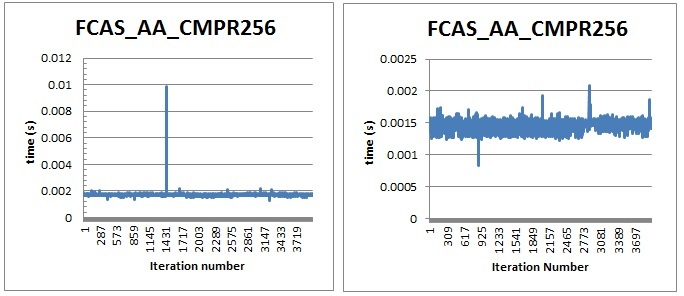
\includegraphics[width=150mm]{figures/chop_off}
	\caption{Before and After Spike Removal}
	\label{fig:mm:chop_off}
\end{figure}
A test run is made to study the effect of background tasks and services on the spikes. The background measurement tasks and services other than \verb|ssh, network-manager| are stopped. Now, only the minimal OS services are running. The Radar application is allowed to run in such less competitive environment. The result shows that the spikes are still occurring in few functional blocks, but the magnitude has reduced from 5x to 2x. As expected, execution time results of some short lived functional blocks do not have the spikes at all. It is concluded that the OS applications or services might have pre-empted the Radar application. Those spikes are removed from the graph and then the maximum execution time is computed. \vspace*{0.2cm}

To effectively utilize all the available four cores, four threads are spawned from main thread to carry out the parallel execution. Core affinity of each thread is set such a way that four threads are mapped to four cores (Appendix \ref{app:code:core_affinity}). For example, thread1 will run on Core\#1, thread2 on Core\#2, thread3 on Core\#3 and thread4 on Core\#4. The Radar application is given higher priority than other user space tasks to give precedence. 

%%%%%%%%%%%%%%%%%%%%%%%%%
%%%%%   SUB-SECTION   %%%
%%%%%%%%%%%%%%%%%%%%%%%%%
\subsection{Memory Transfer Bandwidth}
\label{ss:mm:mem_bw}
Peak achievable memory bandwidth is measured by running threaded STREAM benchmark on Nitrogen6X board. Only STREAM benchmark is started by the user to guarantee that the measurement is not affected by other user applications. 

\lstset{ %
  backgroundcolor=\color{mildyellow},
  numbers=left,
  numberstyle=\tiny\color{mygray},
  frame=single,
  showspaces=false,
  showstringspaces=false,
  basicstyle=\ttfamily,
}

The measurement result of copying data from one memory location to another memory location is used for the  analysis. To measure the peak data transfer rate, the best result from 5 consecutive run is computed. As shown in Table \ref{tbl:mm:bw_no_load}, the iMX6Quad is capable of transferring \textbf{1048 MiB/s} when all the four cores are running in parallel.\\

\begin{table}[h!]
	\centering
	\begin{tabular}{|l|l|} 
	 \hline
	 \textbf{Function} & \textbf{Best Rate [MiB/s]}  \\
	 \hline
	 Copy & 1048.7 \\ \hline
	\end{tabular}
	\caption{Idle Memory Transfer Bandwidth}
	\label{tbl:mm:bw_no_load}
\end{table}

To compute the peak memory bandwidth of the Radar application, STREAM benchmark is allowed to run in background along with the Radar application. STREAM is given low priority to give precedence to the Radar application. When the Radar application is consuming maximum bandwidth, STREAM can only consume the minimum leftover bandwidth. Subtracting minimum recorded bandwidth from the peak memory bandwidth of the iMX6Quad (1048 MiB/s), gives peak memory bandwidth utilized by the Radar application.

%%%%%%%%%%%%%%%%%%%%%%%%%
%%%%%   SUB-SECTION   %%%
%%%%%%%%%%%%%%%%%%%%%%%%%
\subsection{Peak Memory Utilization}
\label{ss:mm:mem_util}
The percentage of the memory being used by a process can be extracted from \bverb|top| command. A bash script(Appendix \ref{app:code:mem_util}) is written to read memory utilization of the Radar application every 10 times a second. The recorded peak memory utilization is exported to an output file for further analysis. This script is also run in background at low priority.

%%%%%%%%%%%%%%%%%%%%%%%%%
%%%%%   SUB-SECTION   %%%
%%%%%%%%%%%%%%%%%%%%%%%%%
\subsection{CPU Utilization}
\label{ss:mm:cpu_load}
CPU utilization is the ratio of busy time to the total time. Busy time is the execution time on a particular CPU and total time is the time delay between two consecutive inputs to the same CPU. The CPU utilization says the percentage of utilization as well as the remaining buffer time for future growth. 50\% spare time is a healthy value for CPU utilization. This spare time can be used for health monitoring that reports hardware and software failures. By doing so, faults can be isolated and stopped from propagating.

\section{Performance Comparison of Single Core vs Four Cores}
\label{sec:mm:perf_comp}
A performance comparison study has been done on the Nitrogen6X board equipped with ARM Cortex A9 quad core processor running functional blocks of the Radar processing algorithm. In Figure \ref{fig:mm:1core_4core}, measurements of 1-thread, CMYACC means running CMYACC functional block on Core\#1 while keeping other cores in idle state. Likewise, measurements of 4-threads states that the CMYACC functional block is executed in all four cores simultaneously. The figure implies that the four core performance is not as good as single core performance. Bottleneck is imposed by the shared resources L2 cache and Memory. In-case more than one core wants to access a shared resource simultaneously, only one core is allowed to access them at a given time. Other cores have to wait until the shared resource is freed again. This increases worst-case execution time of the functional blocks when running on four cores. Although running four cores in parallel does increase the processing time, this thesis sticks to four core version to make use of all the execution resources.

\begin{figure}[h!]
	\centering
	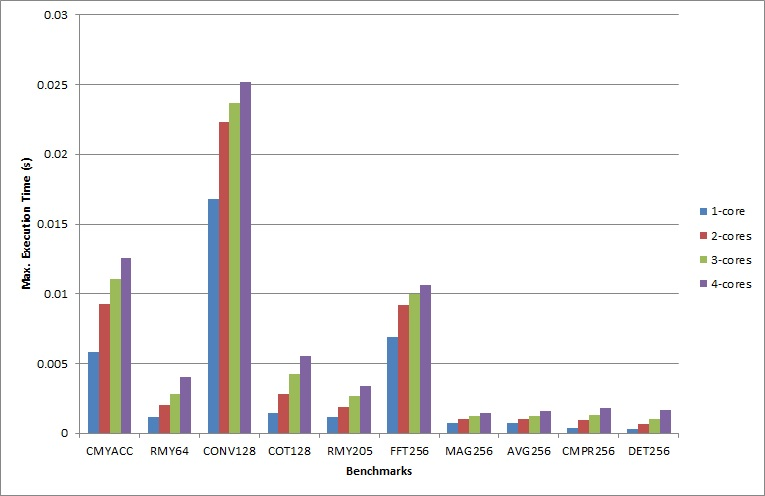
\includegraphics[width=140mm]{figures/1core_4core}
	\caption{Performance of Single Core vs Four Cores}
	\label{fig:mm:1core_4core}
\end{figure}


\clearpage
%%%%%%%%%%%%%%%%%%%%%%%%%%%%%%%%%%%%%
%%%%%%%%%%%%%%%%%%%%%%%%%%%%%%%%%%%%%
%%%%%%%%%%%%   SECTION   %%%%%%%%%%%%
%%%%%%%%%%%%%%%%%%%%%%%%%%%%%%%%%%%%%
%%%%%%%%%%%%%%%%%%%%%%%%%%%%%%%%%%%%%
\section{Design Decisions}
\label{mm:design_decisions}

\subsection{Parallel Execution}
Figure \ref{fig:mm:aa_serial_exe} illustrates the data distribution of Scheme-1 per CPU level. The diagram implies that the nature of execution is serial manner, in other words, it is equivalent to running the application on a single core processor. More CPUs and cores are used to improve the utilization factor, disregarding the processing latency. Thumb rule to reduce the processing latency is to process data independent portions of the application in parallel. 

\begin{figure}[h!]
	\centering
	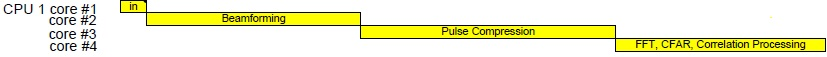
\includegraphics[width=160mm]{figures/aa_serial_exe}
	\caption{Serial Execution of A/A Mode Data in Baseline Analysis}
	\label{fig:mm:aa_serial_exe}
\end{figure}

\subsection{Balanced Utilization}
In all the schemes of the Baseline Analysis, Core\#1 of the A/A Mode CPU does only Input/Output operations, utilizing a smaller amount of the available CPU capability. Due to this, other cores of the CPU have to carry out rest of the processing, leaving them over utilized. This kind of skewed utilization figure pushes up the CPUs worst case utilization factor, so having well balanced utilization is a gesture of a healthy system. Core\#1 should also take part in processing the Radar application for utilization balancing as well as latency reduction. Static scheduling scheme shall be employed to balance the CPU utilization. \vspace*{0.2cm}

\subsection{Space Partition}
Evaluating the results of Time Partition scheme against Space Partition scheme, former one is considered to balance the CPU utilization by defining time slice periods. Down sides of the Time Partition scheme are:
\begin{compactitem} 
\item It magnifies latency by 2x compared to the Space Partition scheme.
\item As it requires breaking the entire application to fit into time slot, it is not scalable (see Chapter \ref{sss:mm:cons:scalability}).
\item Implementation needs more attention when it comes to memory partitioning.
\item Failure of one CPU will affect both the A/A mode and A/G mode processing.
\end{compactitem} 
\vspace*{0.2cm}
To sum up, Time Partition demands more effort and time to realise but producing no better result than Space Partitioning. So, this thesis decides to choose Space Partition as a base for further scheduling schemes.

\subsection{Dedicated Communication Channels}
Distributing the Radar raw data to different CPUs and gathering processed data increases total amount of communication. As depicted in Figure \ref{fig:mm:dedicated_channels}, dedicated channels for input, output between the DGPM and PSM shall be established in Space Partition configuration. It facilitates receiving incoming data stream and sending out processed data simultaneously without interference. The DGPM has 6 port Ethernet interface, of which 4 port shall be connected to 4 CPUs and remaining 2 ports shall act as dedicated input, output channels.

\begin{figure}[h!]
	\centering
	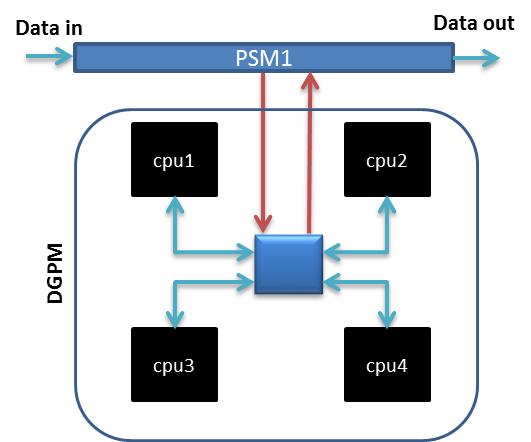
\includegraphics[width=60mm]{figures/dedicated_channels}
	\caption{Dedicated Communication Channels}
	\label{fig:mm:dedicated_channels}
\end{figure}

\subsection{Summary}
In a nut shell, this chapter has scrutinized the Baseline Analysis, discussed the techniques to measure the Radar processor requirement aspects and design choices that should be considered for optimal scheduling.

